\documentclass[11pt,a4paper]{article}

\usepackage{adjustbox}
\usepackage{algorithm}
\usepackage{algorithmic}
\usepackage{amsmath}
\usepackage{amssymb}
\usepackage{amsthm}
\usepackage{amsfonts}
\usepackage{afterpage}
\usepackage{blindtext}
\usepackage[font=footnotesize,labelfont=bf]{caption}
\usepackage{hyperref}
\usepackage[english]{babel}
\usepackage{bbm}
\usepackage{bigints}
\usepackage{bm}
\usepackage{cite}
\usepackage{color}
\usepackage{float}
\usepackage[left=2cm,right=2cm,top=2cm,bottom=2cm]{geometry}
\usepackage{graphicx}
\usepackage[utf8]{inputenc}
\usepackage{mathtools}
\usepackage{mdframed}
\usepackage{pgfplots} 
\usepackage{subfigure}
\usepackage{stmaryrd}
\usepackage{textcomp}
\usepackage{tikz}
\usepackage{url}
\renewcommand{\proofname}{Proof}
\theoremstyle{plain}
\newtheorem{monTheoNumrote}{Théorème}[section] % Environnement numéroté en fonction de la section
\newtheorem*{monTheoNonNumerote}{Théorème}  % Environnement non numéroté
\newtheorem{The}{Theorem}[section]
\newtheorem*{The*}{Theorem}
\newtheorem{Prop}{Proposition}[section]
\newtheorem*{Prop*}{Proposition} 
\newtheorem{Cor}{Corollary}[section]
\newtheorem*{Cor*}{Corollary}
\newtheorem{Conj}{Conjecture}[section]
\newtheorem{Lem}{Lemma}[section]
\renewcommand{\qed}{\unskip\nobreak\quad\qedsymbol}%
\numberwithin{equation}{section} % Numérote les équations section.numéro.
\theoremstyle{definition}
\newtheorem{Def}{Definition}[section]
\newtheorem{Rem}{Remark}[section]
\newtheorem*{Rem*}{Remark}
\newtheorem*{Lem*}{Lemma}
\newtheorem{Que}{Question}
\newcommand{\enstq}[2]{\left\{#1\mathrel{}\middle|\mathrel{}#2\right\}}
\newcommand{\Lp}[2]{L^#1(#2)}
\newcommand{\Sob}[3]{W^{#1,#2}(#3)}
\newcommand{\Rd}[0]{\mathbb{R}^d}
\newcommand{\RN}[0]{\mathbb{R}^N}
\newcommand{\Rn}[0]{\mathbb{R}^n}
\newcommand{\norm}[1]{\left\|#1\right\|}
\newcommand{\sinc}[0]{\textup{sinc}}
\newcommand{\functionDef}[5]{\begin{array}{lllll}
#1 & : & #2 & \longrightarrow & #3 \\
 & & #4 & \longmapsto &\displaystyle #5 \\
\end{array}}
\newcommand{\Theautorefname}{Theorem}
\newcommand{\Propautorefname}{Proposition}
\newcommand{\Corautorefname}{Corollary}
\newcommand{\Lemautorefname}{Lemma}
\newcommand{\Defautorefname}{Definition}
\newcommand{\N}{\mathbb{N}}
\newcommand{\Z}{\mathbb{Z}}
\newcommand{\D}{\mathbb{D}}
\newcommand{\R}{\mathbb{R}}
\newcommand{\A}{\mathcal{A}_{a,b}}
\newcommand{\Crad}{C^\infty_{c,rad}(B)}
\newcommand{\Lrad}{L^2_{rad}(B)}
\newcommand{\Lradab}{L^2_{rad}(\mathcal{A}_{a,b})}
\newcommand{\duality}[2]{\left\langle #1,#2\right\rangle}
\newcommand{\Hrad}{H^1_{rad}(B)}
\newcommand{\Hzrad}{H^1_{0,rad}(B)}
\newcommand{\rmin}{\delta_{\min}}
\newcommand{\rmax}{\delta_{\max}}
\newcommand{\corr}{\gamma}
\newcommand{\question}[1]{\begin{Que} \ 
#1
\end{Que}}
\newcommand{\abs}[1]{\left\lvert #1 \right\rvert}
\newcommand{\CL}[2]{\textup{CL}\left(\enstq{#1}{#2}\right)}
\newcommand{\Script}[1]{`\texttt{#1}`}
\newcommand{\espace}{\text{ }\qquad} 
\newcommand{\loc}{\text{loc}}
\newcommand{\SL}{\textup{SL}\hspace{1.5pt}}
\newcommand{\DL}{\textup{DL}\hspace{1.5pt}}
\newcommand{\fp}{\underset{\varepsilon \to 0}{\textup{f.p.}}}
\newcommand{\scalProd}[2]{\left(#1|#2\right)}
\newcommand{\toDo}[1]{{\color{red}#1}}
\newcommand{\bs}[1]{\boldsymbol{#1}}
\newcommand{\varInRange}[4]{(#1_{#2})_{#3 \leq #2 \leq #4}}
\newcommand{\from}{\colon}
\newcommand{\Cinf}{C^{\infty}}
\newcommand{\isdef}{\mathrel{\mathop:}=}
\newcommand{\defis}{=\mathrel{\mathop:}}

\renewcommand{\algorithmicrequire}{\textbf{Inputs:}}
\renewcommand{\algorithmicensure}{\textbf{Outputs:}}

\pgfplotsset{compat=1.13}
\author{Martin AVERSENG}
\title{Formulaire d'intégrales singulières}
\begin{document}
\maketitle	

\section{$I_0(M) = \displaystyle\int_{[AB]} {\ln|M - Y|d\Gamma(Y)}$}

$A$ and $B$ are two points in the plane. We parametrize the integral according to the figure. A coordinate system is chosen so that $M$ lies on the $y-axis$, with coordinate $M : (0,d)$, and $A$ and $B$ both lie on the $x-axis$, with respective coordinates $A : (a,0)$ and $B : (b,0)$. We let $\overrightarrow{u} = \dfrac{\overrightarrow{AB}}{\abs{AB}}$ and $\overrightarrow{n}$ a couple of unit tangent and normal vector of the segment $[AB]$. This way, we have $a = \overrightarrow{MA}\cdot \overrightarrow{u}$, $b =  \overrightarrow{MB}\cdot \overrightarrow{u}$, and $d = \abs{\overrightarrow{AM} \cdot \overrightarrow{n}}$ (the integral is unchanged by changing the orientation of $\overrightarrow{n}$).
\begin{figure}[H]
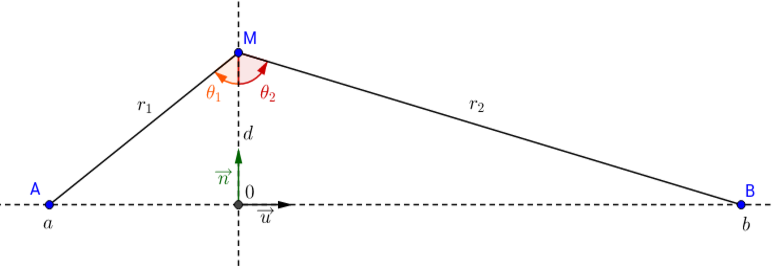
\includegraphics[width=0.9\textwidth]{figureIntegraleSinguliere}
\caption{Parametrization for the computation of $I_0(M)$}
\label{fig:figureIntegraleSinguliere}
\end{figure}

According to this choice of parametrization,
\begin{align*}
	I_0(M) &= \int_{a}^b \ln \sqrt{y^2 + d^2} dy\\
	& = \left[y \ln \sqrt{d^2 + y^2}-y +d \arctan{\frac{y}{d}}\right]_a^b\\
	&= b \ln r_2 - a \ln{r_1} - |AB| + d (\theta_2 - \theta_1)
\end{align*}

By continuity of the single layer potential, the value of $I_0(M)$ for $M$ aligned with $A$ and $B$ is obtained by sending $d$ to $0$. If $M$ is in the segment, $\theta_2 - \theta_1 = \pi$, while it is $0$ otherwise. 

\section{$I_1(M) = \displaystyle\int_{[AB]} {\ln|M - Y|\phi_1(Y)d\Gamma(Y)}$}

The function $\phi_1$ is an affine function of $Y$. Using the same parametrization as previously, and taking $\phi_1(y) =  \alpha y + \beta$, we need only compute the integral $I_{1} = \displaystyle \int_{a}^b y \ln \sqrt{d^2+ y^2}y$. 
We have
\begin{align*}
	I_1 &= \left[\frac{1}{2} \ln \sqrt{d^2 + y^2} (d^2 + y^2) - \frac{1}{4}(d^2 + y^2)\right]_a^b\\
	&=  \frac{1}{2} \left( r_2^2 \ln r_2  - r_1^2 \ln r_1\right)  + \frac{1}{4}\left(r_2^2 - r_1^2\right)
\end{align*}
	
Accordingly, 
\begin{align*}
	I_1(M) &= \alpha I_1 + \beta I_0(M)\\
	&=  \frac{\alpha}{2} \left( r_2^2 \ln r_2  - r_1^2 \ln r_1\right)  + \frac{\alpha}{4}\left(r_2^2 - r_1^2\right) + \beta\left[b \ln r_2 - a \ln{r_1} - |AB| + d (\theta_2 - \theta_1)\right]\\
\end{align*}



\end{document}